\documentclass[11pt]{article}
\usepackage[margin=1in]{geometry}
\usepackage{graphicx}
\usepackage{hyperref}
\usepackage{float}
\usepackage{parskip}

\title{QSS 20 Final Project Milestone 1}
\author{Alanna Polyak}
\date{Last updated: August 3, 2026}

\begin{document}
\maketitle

\section{Project Option}

\textbf{Senior Thesis / Own Data.} I am pursuing an own-data project on the
mismatch between where the burden of neurological and neurodegenerative disease
falls and where the workforce capable of diagnosing and managing that disease
actually exists. The unit of analysis is the country. The project assembles
three sources: the WHO/World Federation of Neurology \emph{Atlas: Country
Resources for Neurological Disorders} (2nd ed., 2017), which reports
neurological workforce density and service availability for 133 countries and
territories; the IHME Global Burden of Disease (GBD) study, which supplies
country-year estimates of neurological disease burden in DALYs, prevalence, and
incidence; and the Demographic and Health Surveys (DHS), which supply
population-level demographic and health-system covariates and, through the
geographic datasets, cluster-level information on distance to care. This
milestone works with the Atlas data, which I have already extracted and cleaned;
the GBD and DHS extracts are in progress (see Section~\ref{sec:data}). The
project is deliberately scoped as Part~1 of a two-part design: the country-level
access gradient estimated here is intended to enter a separate household-level
analysis of informal caregiving reliance as a contextual predictor.

\section{Your project's main questions}

The project asks three linked questions. First, descriptively, how large is the
gap between neurological disease burden and neurological workforce capacity, and
how does that gap vary across World Bank income groups and WHO regions? Second,
is the gap better characterized as a national scarcity problem or as a
distributional problem within countries---that is, do countries with low
aggregate workforce density also concentrate what workforce they have in capital
cities, so that the effective access gap for a rural resident is substantially
worse than the national density figure implies? Third, once income group and
demographic structure are accounted for, does residual variation in workforce
density predict anything about how neurological need is met outside the formal
health system? I do not expect to identify a causal effect of workforce density
on outcomes; the ambition is to construct a defensible, reproducible measure of
the burden--capacity gap and to characterize its structure, which is a
prerequisite for the household-level question rather than an answer to it.

\section{Your project's data sources/relevant fields}
\label{sec:data}

The WHO/WFN Neurology Atlas is the workforce source. I extracted two tables
directly from the published PDF. The first is the participating-country annex,
which yields 133 rows with fields \texttt{country}, \texttt{who\_region}, and
\texttt{wb\_income\_group}; this serves as the crosswalk onto which the other
sources merge. The second is the results tables (Tables 2--3, Figures 11--12,
15--16), which give, by income group and by WHO region, the median total
neurological workforce per 100\,000 population, disaggregated medians for adult
neurologists, neurosurgeons, and child neurologists, the number of responding
countries behind each median, and the share of countries reporting that
neurologists practise in the capital city, in other urban areas, and in rural
areas. The Atlas is a survey of ministry-of-health focal points, so response
counts vary by item (114 countries for workforce density, 93 for child
neurologists), and this variation has to be carried through the analysis rather
than ignored. The IHME GBD extract will supply \texttt{location\_name},
\texttt{year}, \texttt{cause\_name}, \texttt{measure\_name} (DALYs, prevalence,
incidence), \texttt{metric\_name} (rate per 100\,000 and number), and
\texttt{val}/\texttt{upper}/\texttt{lower}, restricted to the Level~2
neurological disorders cause group and its Level~3 children (stroke, dementias,
epilepsy, Parkinson disease, migraine) for all countries. The GBD file currently
in hand is a global all-cause summary and is not usable at the country level; it
is being re-pulled at country resolution. DHS will supply population age
structure, urban/rural residence, and health-service utilization indicators, plus
GPS cluster coordinates for the distance-to-facility component; the DHS
application is pending authorization.

\section{Create one starter visualization}

Both figures below are built from the Atlas data described above using pandas and
matplotlib. Figure~\ref{fig:one} establishes the aggregate scarcity gradient.
The median total neurological workforce is 0.1 per 100\,000 population in
low-income countries against 7.1 in high-income countries---a 71-fold difference,
and the gap is wider still for adult neurologists specifically (0.03 versus 4.75,
roughly 158-fold). Two of the four income groups sit below the global median of
3.1, and the low-income median is close enough to zero that a country-level
regression on this outcome will be badly skewed and almost certainly needs a log
or rank transformation.

\begin{figure}[H]
\centering
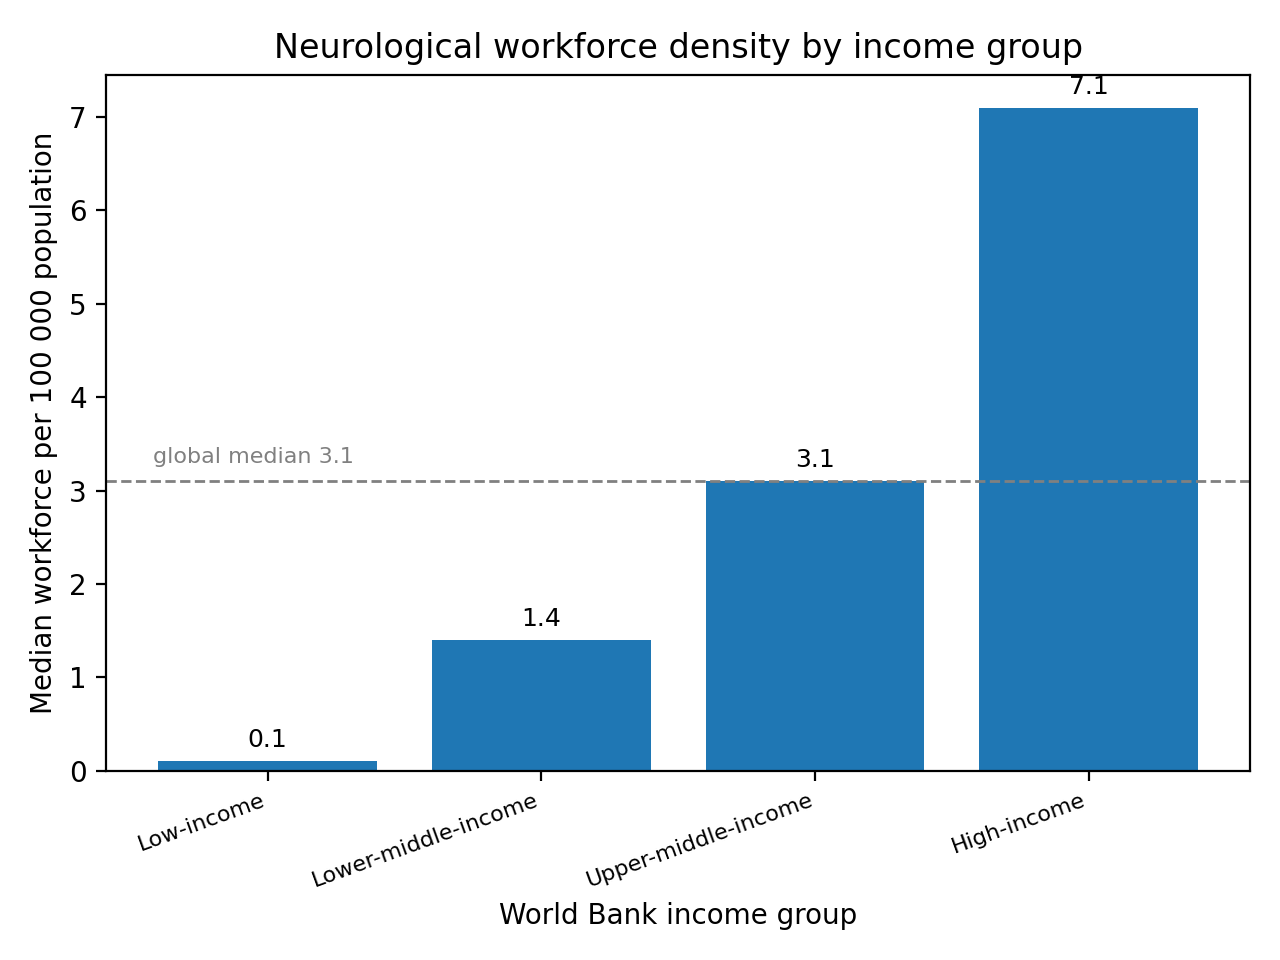
\includegraphics[width=0.8\textwidth]{figures/fig1_workforce_by_income.png}
\caption{Median neurological workforce per 100\,000 population by World Bank
income group. Source: WHO/WFN Neurology Atlas, 2nd ed. (2017), Fig.~12;
$N=114$ responding countries.}
\label{fig:one}
\end{figure}

Figure~\ref{fig:two} is the one that motivates the project's second question.
Reading across income groups, the share of countries reporting neurologists in
the capital city is essentially flat---95\% to 100\% everywhere---while the share
reporting any neurologist practising in rural areas falls from 45\% in
high-income countries to 0\% in low-income countries. In other words, the
national density figures in Figure~\ref{fig:one} understate the problem: in the
poorest countries the entire specialist workforce is urban, so a rural resident
faces an effective density of zero regardless of what the national median says.
This is the specific pattern the DHS geographic data is intended to quantify.

\begin{figure}[H]
\centering
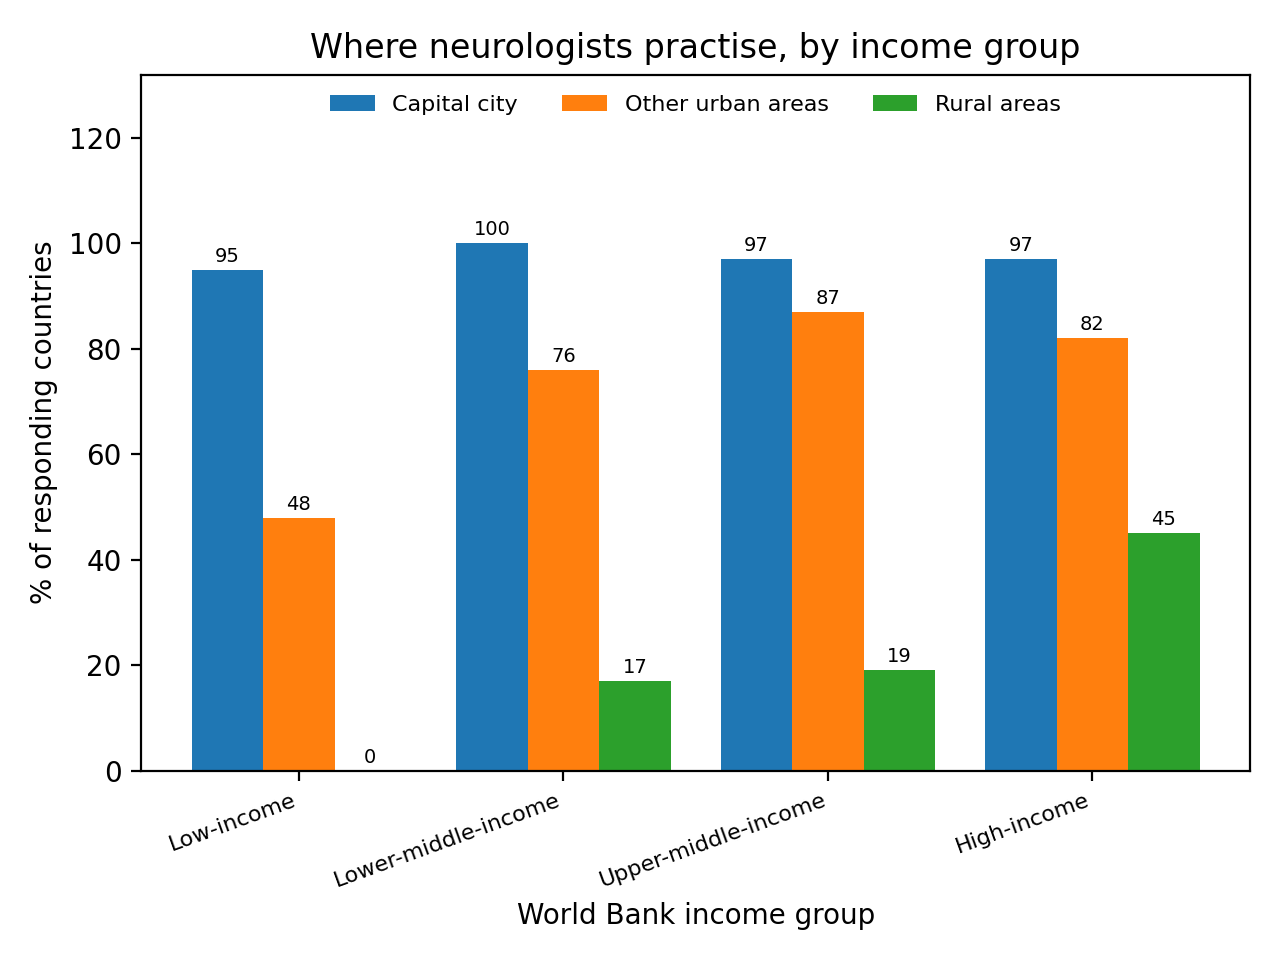
\includegraphics[width=0.8\textwidth]{figures/fig2_where_neurologists_practise.png}
\caption{Share of responding countries reporting that neurologists practise in
each setting, by World Bank income group. Source: WHO/WFN Neurology Atlas, 2nd
ed. (2017), Fig.~16; $N=114$ responding countries.}
\label{fig:two}
\end{figure}

\section{Learn from an earlier project on your research topic}

I read the descriptive comparison example on felony sentencing: Fink, Jin,
Punaini and Tolat's study of racial disparities in Cook County bail decisions.
The substantive topic is unrelated to mine, but the structure is nearly
identical---a descriptive comparison of outcomes across groups, drawn from
administrative data, where the quantity of interest is a gap and the central
threat is confounding the data cannot resolve.

The lesson I take concerns their choice of comparison units. They never compare
Black and White defendants in the aggregate. Every analysis first subsets to a
specific offense category---Armed Robbery, Homicide, Unlawful Use of Weapon,
Robbery, Battery---on the reasoning that a pooled comparison would mostly reflect
differences in charge composition rather than differential treatment of similar
cases. Equally useful is their insistence on reporting a disparity on two scales
at once. In their Table 8, bond-increase rates differ across race by as little as
0.0006 in absolute terms while differing by factors of 1.25 to 8 in relative
terms; on either scale alone the finding would be badly misleading. I intend to
import both habits. Workforce density should never be compared across countries
without conditioning on income group, and the burden--capacity gap should be
reported in absolute and relative terms together, since the low- versus
high-income contrast in adult neurologist density is a 4.7-point absolute gap per
100\,000 population and simultaneously a 158-fold relative one.

The weakness I want to improve on is that they identify their central confounder
and then proceed as though naming it discharged the obligation. Criminal history
is unavailable in their data, and they say so plainly---in the Methods section,
and again in the Limitations section---but it never re-enters the analysis. There
is no bounding exercise, no sensitivity analysis, and no attempt to ask how large
the unmeasured confounding would have to be to erase the disparities they report.
The reader is left holding a stated caveat and a table of point estimates with no
way to reconcile them. A related gap: they report $p$-values for Table 2 but not
for Tables 3 through 8, and the relative differences in Table 8 rest on rates
between 0.0001 and 0.0015, so an eight-fold ratio may be built on a handful of
cases with no counts or intervals shown. Their inner join also retains only 45\%
of case participants, a selection they speculate about but never test.

My analysis faces the structurally identical problem: national income drives both
neurological workforce capacity and measured disease burden, and measured burden
additionally depends on the diagnostic capacity that is my exposure. I plan to
improve on their treatment in two concrete ways. First, every estimate will carry
its denominator---Atlas response counts already vary from 93 to 114 countries by
item, and my merged file will keep a per-country coverage indicator for each
source rather than silently dropping incomplete rows. Second, income will be
modeled and bounded rather than merely disclosed: stratified estimates within
income group, plus an explicit statement of how large a confounding effect would
need to be to overturn the observed gap. Naming a confounder in the limitations
section is not the same as accounting for it.

\section{Your project's anticipated challenges}

The pre-mortem has four entries. The first is measurement: ``neurological
workforce'' in the Atlas is a self-reported count from a ministry focal point,
with no auditing, no full-time-equivalent adjustment, and no guarantee that
countries applied the glossary definitions consistently, so cross-country
comparisons are noisier than the clean medians suggest. The second is
missingness, and it is almost certainly not missing at random: the countries that
failed to respond to the Atlas survey are plausibly those with the weakest health
information systems and therefore the weakest neurological services, which would
bias any complete-case analysis toward understating the gap. I plan to handle
this with explicit missingness indicators and sensitivity analysis rather than
imputation that assumes MAR. The third is temporal and unit alignment: the Atlas
reflects 2014--2015 data collection, GBD estimates are annual through 2023, and
DHS surveys are fielded country-by-country on irregular cycles, so any merged
panel will require deliberate decisions about which year to anchor on and will
have ragged coverage. Country-name harmonization across three sources with three
different naming conventions is a related and tedious risk. The fourth is
causality, and here I want to be disciplined up front: workforce density,
disease burden, and national income are so tightly entangled---income affects
both capacity and measured burden, and measured burden depends on diagnostic
capacity, which is the exposure---that any estimate framed as the effect of
workforce on outcomes would be uninterpretable. The project is therefore framed
descriptively, and the burden--capacity gap is treated as a construct to be
measured well rather than a treatment to be estimated.

\end{document}
